%!TEX root = main.tex
%
% Start with sampling patterns 
%
%
\begin{figure}
\begin{tabular}{c c c}
\multicolumn{3}{c}{samples on a regular grid (biased and consistent)}\\
%   \begin{sideways} regular (biased) \end{sideways} & 
  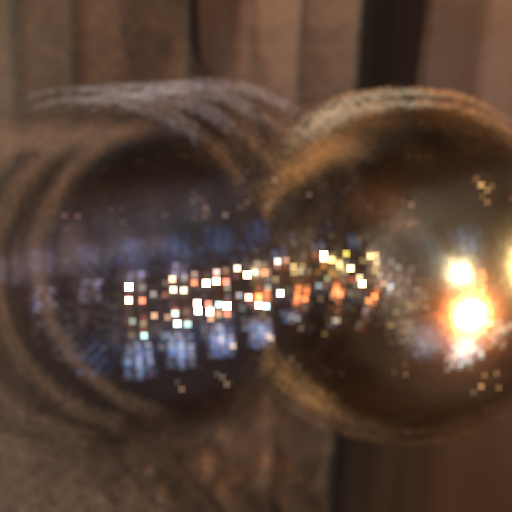
\includegraphics[width=.3\linewidth]{../PBRTOut/pngs/testmb_ball.scene_GRID_2_Samps_iter_1_1_uj.exr.png}&
  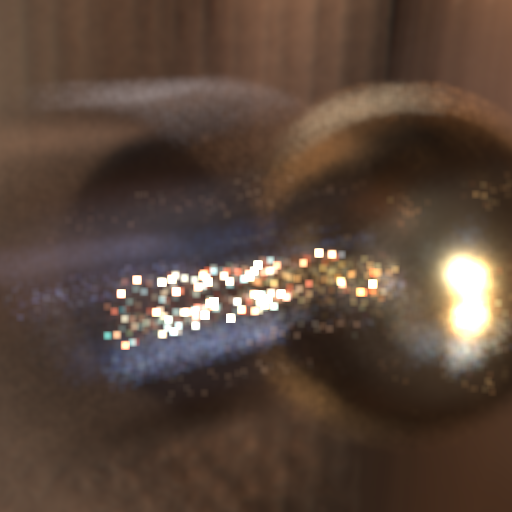
\includegraphics[width=.3\linewidth]{../PBRTOut/pngs/testmb_ball.scene_GRID_4_Samps_iter_1_1_uj.exr.png}&
  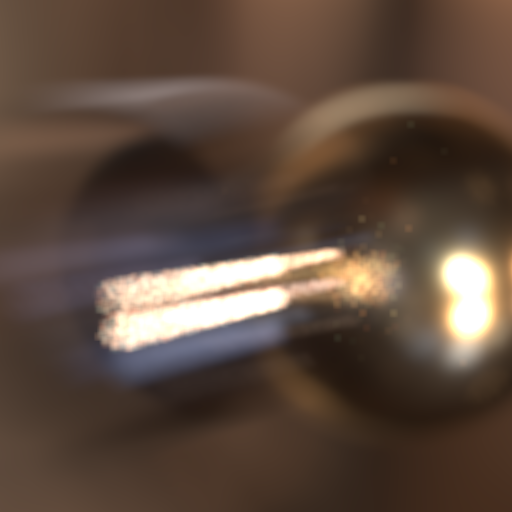
\includegraphics[width=.3\linewidth]{../PBRTOut/pngs/testmb_ball.scene_GRID_64_Samps_iter_1_1_uj.exr.png}\\
  \hline
\multicolumn{3}{c}{low-discrepancy sampler (biased and consistent)}\\
%     \begin{sideways} low discrepancy (biased) \end{sideways} &
  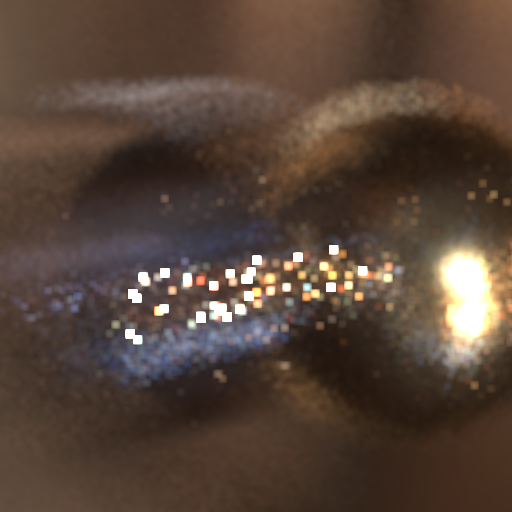
\includegraphics[width=.3\linewidth]{../PBRTOut/pngs/testmb_ball.scene_LD_4_Samps_iter_1__uj.exr.png}&
  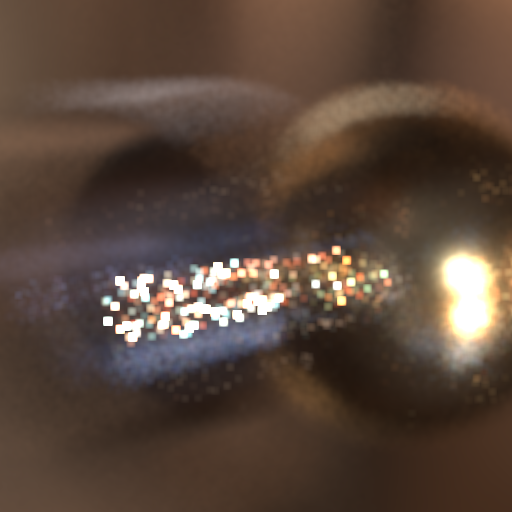
\includegraphics[width=.3\linewidth]{../PBRTOut/pngs/testmb_ball.scene_LD_16_Samps_iter_1__uj.exr.png}&
  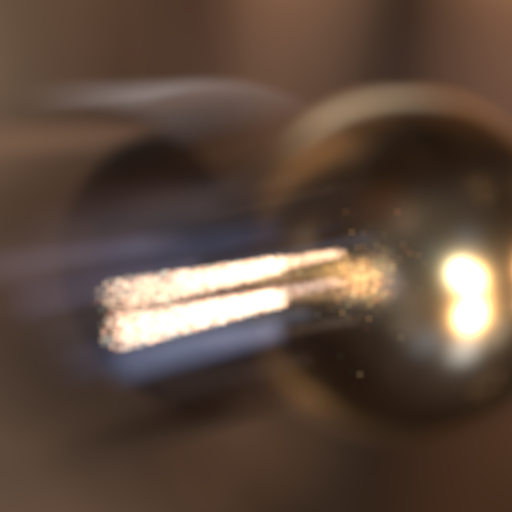
\includegraphics[width=.3\linewidth]{../PBRTOut/pngs/testmb_ball.scene_LD_4096_Samps_iter_1__uj.exr.png}\\
\hline
\multicolumn{3}{c}{random sampling (unbiased and consistent)}\\
%     \begin{sideways} random (unbiased) \end{sideways} &
  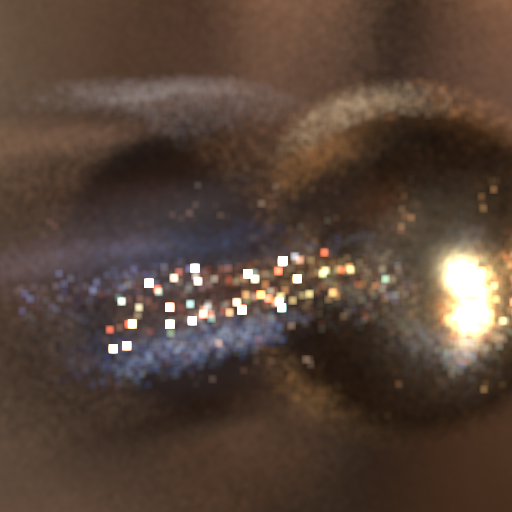
\includegraphics[width=.3\linewidth]{../PBRTOut/pngs/testmb_ball.scene_RAND_4_Samps_iter_1__uj.exr.png}&
  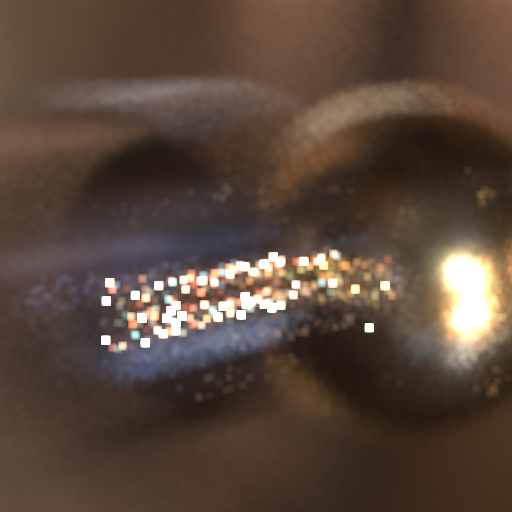
\includegraphics[width=.3\linewidth]{../PBRTOut/pngs/testmb_ball.scene_RAND_16_Samps_iter_1__uj.exr.png}&
  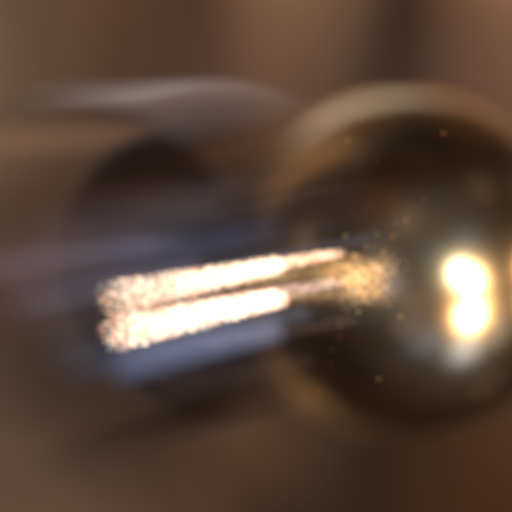
\includegraphics[width=.3\linewidth]{../PBRTOut/pngs/testmb_ball.scene_RAND_4096_Samps_iter_1__uj.exr.png} \\
   4 samples per pixel (spp)& 16 spp& 4096 spp \\
\end{tabular} 
\caption{\label{fig:errorrender}
A comparison of rendered results obtained using 3 sampling strategies (rows) for various sampling counts (columns). The images depict two shiny balls: A golden ball that is out of focus and a mirrored ball  that is moving rapidly through the plane in focus. All strategies lead to consistent estimators, therefore the images in the third column are virtually indistinguishable. The na\"ive, biased strategy of sampling on a regular grid leads to objectionable visual artifacts. A more sophisticated approach --- low-discrepancy sampling (middle row) --- although biased, not only eliminates the regular artifacts but also exhibits improved noise characteristics (for example in the background region, using 16 samples) compared to unbiased estimates obtained using random sampling (bottom row). }
\end{figure}

\subsection{Manifestation of error in rendering}
For a given scene configuration (hence fixed integrand), the error in the rendered image is primarily dependent on the choice of sampling strategy. To a lesser extent, the error also depends on the algorithm used for rendering (path-tracing, Metropolis light transport, etc.). The motivation behind using stochastic sampling over regular samples was related to human perception. The bias caused by using regularly placed samples is considered more objectionable~\cite{Wold85,Cook:1986:SSC} to our visual systems than its appearance as noise that is distributed across all frequencies (compare the strategies in the first column of fig.~\ref{fig:errorrender}). 

Consider an image rendered using path tracing with 64 samples per pixel. Each pixel in the final image can be viewed as a single instance of a secondary estimator, of the integral corresponding to that pixel, using 64 samples. In theory, the variance of each of these estimates can only be observed by rendering multiple images with 64 samples per pixel. In practice, even though the integrand at each pixel is different, the radiance varies smoothly over many parts of the image. As a result, if estimators for pixels in these smooth regions have high variance, their disagreement on particular instances of the estimate (in the rendered image) leads to a noisy appearance. The larger the disagreement of estimates in neighboring pixels in smooth regions, the noisier the image will appear. In other words, an estimator with a higher variance will lead to a noisier image.

The manifestation of bias is less intuitive. Typically, estimators with a structured bias --- such as one that uses a regular sampling pattern --- produce banded visual artifacts. In some cases, bias leads to artifacts that are inconsistent with our expectation of realism.~e.~g.~bright patches at points where contact shadows are expected. Bias may also lead to incorrect estimates where the error is not visually perceivable. Such estimators are desirable, particularly if they can simultaneously improve the visual noise. The solution to the inveterate problem of striking a reasonable compromise between bias and variance, for efficiency, depends on the nature of the scene, choice of sampling strategy, number of samples, etc. 

The reduction of error, for a given sampling strategy, might be achieved by increasing the number of samples. So, in the above example, rendering with 128 or 256 samples per pixel will reduce noise. 
% The rapidity with which variance diminshes, as the number of samples is increased, is called the \textit{convergence rate} of the estimator. 
Some estimators (jittered sampling, QMC sampling) converge faster than others. Even for a fixed sampling strategy, primary and secondary estimators have different distributions and hence different statistics. Secondary estimators approach being Gaussian-distributed, as the number of the fixed samples used is increased. Choosing the ``best'' estimator depends on the application. For high-quality, offline rendering the estimator of choice will be the one with the quickest convergence. On the other hand, for applications with a time-budget, the estimator with the lowest error for the given budget of samples must be chosen.



